\toclesssection{SCP 020 - Unseen Mold}
\addcontentsline{toc}{section}{SCP 020 - Unseen Mold}

\textbf{Item \#:} SCP-020

\textbf{Object Class:} Keter

\begin{figure}[h]
\begin{center}
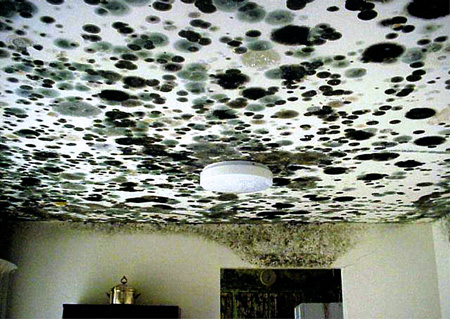
\includegraphics[scale=0.6]{scp/020a.jpg}
\linebreak SCP-020 growths in a civilian residence.
\end{center}
\end{figure}

\textbf{Special Containment Procedures:} Samples of SCP-020 are kept in a hermetically sealed cylindrical cultivation chamber measuring 1 m in diameter and 1 m high. This chamber is located inside a sealed containment room, accessible only via airlock. Nutrients are administered via automated robotic systems, as the cultivation chamber must remain sealed at all times.

Hermetically sealed video surveillance cameras are installed within the containment room, and must be checked daily for integrity. Any personnel entering the containment room must undergo a full anti-fungal disinfection procedure upon exiting.

\textbf{Description:} SCP-020 is a fast-spreading fungal organism that is capable of affecting the senses and behavior of living creatures, including humans. Samples of SCP-020 exhibit an unknown effect that renders them effectively invisible to direct observation, even when under a microscope. SCP-020 is only visible to humans when viewed through photographic or video surveillance.
\newpage
Once SCP-020 forms a colony, usually within a human residence, it will produce spores that affect the behavior of humans around it. Affected subjects will increase the heat and humidity within their homes to create an environment more suitable to the growth of SCP-020. Affected subjects also become more sociable in many cases, and often invite acquaintances to their homes to further spread the organism. As the spores and mold colonies are invisible to affected subjects, the mold may sometimes grow directly on living subjects.

\begin{figure}[h]
\begin{center}
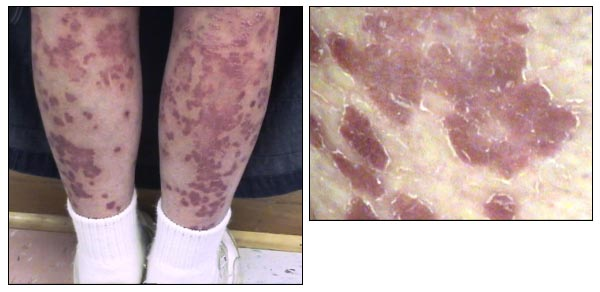
\includegraphics[scale=0.5]{scp/020b.jpg}
\linebreak A civilian infected with SCP-020 colonies.
\end{center}
\end{figure}

As the spores and colonies within a home approach critical concentration, the health of affected human subjects will rapidly deteriorate, resulting in death. Further spread of the mold may occur as the bodies of any deceased subjects are encountered by emergency responders and health care agents, as well as transportation of the bodies to local morgues.

SCP-020 was first encountered in \expunged, where an undercover SCP agent noted dramatic personality changes in personnel working at the local hospital. Upon investigation by a containment team, it was discovered that almost \censor{XXX} civilians had been infected, as well as a majority of the town. The civilian population was terminated, and the town incinerated under cover of a local flash forest fire.

To date, over 12 outbreaks of SCP-020 have been reported. Investigations are currently underway to determine the source of these outbreaks and possible preventative measures.

\textbf{Addendum 020-01:} Excerpts from the audio/video mission recorders of Mobile Task Force \expunged \ during the initial containment of SCP-020 at \expunged.

\begin{leftbar}
\begin{flushleft}

\textbf{T2-Lead:} Team Two moving to the red house.\linebreak
\textbf{T2-COM:} Copy, UAV One is picking up one heat signature.\linebreak

...\linebreak

\textbf{T2-Lead:} Team Two in place, ready to br- \lb Expletive\rb!\linebreak
\textbf{T2-2:} The door's opening!\linebreak

\textsl{At this point, a civilian woman appeared in the doorway, holding a kitchen knife. Video surveillance showed that nearly two-thirds of her face was covered by mold growths.}\linebreak

\textbf{Civilian Woman:} Well... hello there, gentlemen... care to take a breather inside?\linebreak
\textbf{T2-Lead:} On the ground! Drop the weapon!\linebreak
\textbf{Civilian Woman:} Don't be silly! Come on in and... stay a while...\linebreak
\textbf{T2-Lead:} Stop where you are! DROP THE WEAPON!\linebreak
\textbf{Civilian Woman:} We... we just want to have some guests... please... come in...\linebreak
\textbf{T2-2:} Drop the \lb Expletive\rb \ weapon!\linebreak

\textsl{It is assumed that at this point, the infected civilian noticed T2-4 carrying a primed incendiary weapon, and lunged forward at the team members with the knife.}\linebreak

\textbf{Civilian Woman:} \expunged \linebreak
\textbf{T2-Lead:} Open fire, open fire!\linebreak

\textsl{Gunfire, screaming.}
\end{flushleft}
\end{leftbar}